\documentclass[]{article}
\usepackage{cite}
\usepackage{graphicx}
%opening
\title{Temporal Map of Healthcare in Nigeria}
\author{Kyle Shan}

\begin{document}

\maketitle

\begin{abstract}
We explore using publicly available satellite images from Landsat 8 to predict vaccination rates in Nigeria. We use Google Earth Engine to produce a composite image and export patches centered at DHS clusters. These images are used as input to a convolutional neural network, which produces feature vectors describing each image. To avoid training on a small dataset, we first train the network to predict nighttime light intensity, a proxy for overall expenditure, at many points around DHS clusters. We then fine-tune this network to predict vaccination rates, attaining over 70\% R-squared for some vaccines on a holdout set. We use Integrated Gradients and t-SNE embedding to visualize the network, as well as regression analysis with several proxies for expenditure. Based on our analysis, the model appears to make predictions based on economic indicators that can be identified from the satellite images.
\end{abstract}

\section{Introduction}
In several African countries, children do not have access to routine immunizations, resulting in a large burden of vaccine-preventable diseases such as polio or measles. In order to improve vaccine coverage, policymakers need to know which areas have low vaccination rates. However, this information is not always readily available. The Demographics and Health Surveys (DHS) program \cite{dhs2014} conducts surveys infrequently - every 5 years  - and not all areas are covered by these surveys. Creating a predictive model for vaccination rates based on publicly available and frequently collected data can permit more effective policy decisions.

Recent research in computer vision has shown that convolutional neural networks (CNNs) can be trained to recognize various characteristics, such as poverty \cite{jean2016combining} and land usage \cite{castelluccio2015land}, using satellite images. The use of satellite images is appealing because these images cover much of the world, are updated frequently, and are publicly available. In last year's IDM Xplore project \cite{zhan2019}, Ruohan Zhan and Yuan Gao used a CNN model trained by Jean et al. \cite{jean2016combining} to predict healthcare outcomes, including vaccination rates, using satellite images from Google Static Maps. Images from Google Static Maps have high quality and resolution, but only the most recent composite is available. Perez et al. \cite{perez2017poverty} found that using images from the Landsat 7 satellite can produce comparable or better predictive accuracy than Google Static Maps; Landsat 7 images have a lower resolution, but contain data from sensors that detect beyond the visible spectrum.

Consequently, we hypothesize that using images from Landsat satellites can also allow us to predict vaccination rates, with a few notable advantages. First, as Perez et al. note, Landsat images are available going back decades, allowing us to make a temporal map of predictions. Second, the Landsat 8 satellite, which began operation in 2013, has improved sensors compared to Landsat 7, and does not suffer from the Scan Line Corrector malfunction that occurred in Landsat 7 \cite{slc2003}, so performance with Landsat 8 could be higher than using Google Static Maps. Third, the lower spatial resolution of Landsat 8 images results in lower computational requirements than using Google Static Maps.

\section{Data and Processing}
We use several data sources in this project, all of which are publicly available. Our efforts are focused on predicting vaccination rates in Nigeria. Nigeria has not had as much political turmoil as other countries with low vaccination rates, which would otherwise introduce additional uncertainty in predicting healthcare.

\subsection{DHS Surveys}
For data on vaccination rates, we use the most recently available DHS questionnaire, which is the DHS phase 6 conducted in 2013 \cite{dhs2014}. We try to predict the vaccination outcomes from the household surveys, where the household parents answer questions about their children's vaccination status. Parents may have a health card for their children, which verifies when their children receive vaccines; however, we treat any affirmative response, regardless of whether the parents have the health card, as a true vaccination. Responses of ``don't know'' and missing responses are discarded. Each household is assigned by DHS to a survey cluster; we summarize the vaccination rates for each cluster. The locations of these clusters are randomly shifted by DHS, by up to 5km for most locations.

\subsection{Satellite Images}
We use Google Earth Engine to combine multiple satellite images taken of each spatial location, producing a single composite raster for each data source. Using the Python API, we can define 25km square regions centered at each DHS cluster and export the corresponding patches of the composite image. We use the following data sources:
\begin{itemize}
\item Landsat 8 \cite{landsatSite}. We use pixel-level cloud coverage data to mask cloud pixels, and then produce a composite of cloud-free pixels by taking the median pixel values for each band over a three-year period (Jan 2013-Dec 2015). Although it would be ideal to only use images taken around the time of the DHS survey, some areas are frequently cloudy - even though the Landsat 8 satellite revisits each image location every 8 days, there are some areas that have no cloud-free pixels even in the three-year span. We use bands 1, 2, 3, 4, 5, 6, 7, 10, and 11 from the Landsat 8 sensors; see \cite{landsatSite} for band details.
\item Global Human Settlement Layers (GHSL) \cite{ghsl}. This is a raster of built environment, which is produced by a model that segments Landsat images into water, not built, and built.
\item DMSP OLS Nighttime Lights \cite{dmspols}. This is a collection of nighttime images which captures nighttime light intensity. 
\end{itemize}

\section{Methods}
Following the methodology of \cite{jean2016combining}, we produce our model in two steps. 

\subsection{Feature Extractor}
First, we train a CNN to predict nighttime light intensity from Landsat 8 composites. Since these datasets are available across all of Nigeria, we can sample far more examples than just the DHS. This additional data availability is crucial; we cannot rely on pretrained models (e.g. on ImageNet), since our input contains 9 input channels instead of the usual 3.

Light intensity from the DMSP OLS dataset is measured from 0 to 63. While \cite{jean2016combining} defines low, medium, and high light intensity with cutoffs at 2.5 and 34.5, we find that these cutoffs produced too many images with a median intensity level of ``medium'', so we adjust these cutoffs to 3.5 and 15.5, resulting in equally log-spaced buckets. Figure \ref{fig:nightlight} shows information about the distribution of night light intensities. Using these light intensities, we intend to train CNNs to classify Landsat images into low/medium/high nightlight intensity using cross-entropy loss.

\begin{figure}[t]
\centering
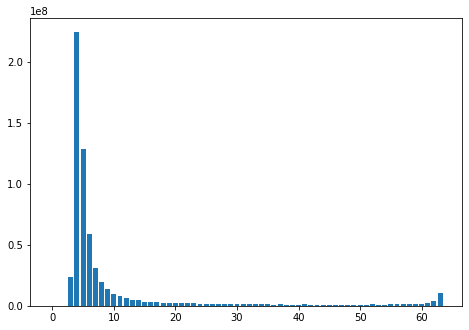
\includegraphics[width=.4\linewidth]{nightlight_hist.png}
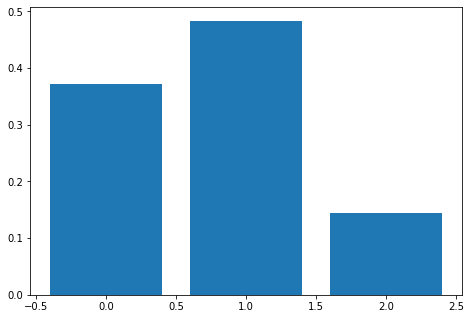
\includegraphics[width=.4\linewidth]{nightlight_buckets.png}
\caption{On the left, the distribution of nightlight intensities for pixels in our image dataset. On the right, the distribution of low, medium, and high intensity images, as determined by taking the median intensity of pixels in the image and bucketing into the ranges 1-3, 4-15, 16-63.}
\label{fig:nightlight}
\end{figure}

We use 10km square patches as the input to our model. To avoid sampling many rural areas with very low light intensity, we focus on areas close to DHS clusters. This is done by sampling 25km square patches centered at each cluster; we randomly crop a 10km square (333 pixels at the Landsat 8 resolution of 30m/px). We also apply a random horizontal flip and 90-degree rotation as data augmentation. Lastly, each channel of the input is normalized based on the sample mean and standard deviation of the images in our dataset.

To avoid excessive computational requirements, we test relatively lightweight CNN architectures: VGG \cite{simonyan2014deep}, ResNet \cite{he2015deep}, and MobileNet v2 \cite{Sandler_2018}. Implementations are those included in the Torchvision \texttt{models} subpackage of PyTorch \cite{paszke2017automatic}. We modify the first convolutional layer of each architecture to take 9 input channels rather than the usual three red/green/blue. For VGG, while the original architecture reshapes the 512-channel feature map to produce a very high-dimensional feature space, we instead average-pool this feature map to produce only 512 output features. Some of these architectures have a multiple-hidden-layer fully connected network after the convolutional layers; we replace these with only a single fully connected layer in all cases.

Models are trained on a Windows machine with a GTX 1070 GPU, using a batch size of 32 images, 50 epochs, and the Adam optimizer \cite{kingma2014adam}.

\subsection{Predictor}
After training the feature extractor, we apply it to a 10km square center-crop of the 25km square patches with no data augmentation. This yields a dataset of feature vectors, which we will use to predict vaccination rates. We could use any supervised method here, but using a neural network will allow us to combine the feature extractor and predictor to form an end-to-end neural network pipeline.

We train neural networks with one or two hidden layers to predict vaccination rates with binary cross-entropy loss. Since our data is at the cluster level, we weight the loss by multiplying by cluster population. The model is trained to predict all vaccine-related outcomes simultaneously, with the corresponding losses weighted equally. We use a batch size equal to the number of data points and iterate for 400 epochs. For hyperparameter validation, the dataset is randomly split 80/20 into a training and test set, and we report the test set accuracy.

\subsection{Model Interpretation}
Beyond predictive accuracy, we are also interested in the visual features identified by the model. First, we use Integrated Gradients \cite{sundararajan2017} to estimate the importance of each pixel in the inputs. This method produces a heatmap of pixel importance, highlighting the pixels of the image which have the most influence on the prediction. Another visualization method is to embed the extracted features in two-dimensional space using t-SNE embedding \cite{vanDerMaaten2008}, and then show the images in a 2D grid. This gives a rough idea of which images are considered similar.

\section{Results}
In this section, we first describe the predictive accuracy of our model, and then explore various methods of CNN visualization.

\begin{table}[t!]
\centering
\begin{tabular}{c | c}
\hline
Architecture & Accuracy \\
\hline
ResNet-34 & 76\% \\
VGG11 & 80\% \\
VGG16 & 78\% \\
MobileNet V2 & 72\% \\
\hline
\end{tabular}
\caption{Classification accuracy of various architectures for nighttime light intensity.}
\label{table:extractor}
\end{table}

\begin{table}[t!]
\centering
\begin{tabular}{c | c c | c}
\hline
Outcome & Training R2 & Test R2 & Gao \& Zhan \\
\hline
bcg&79\%&72\%&64\%\\
measles&65\%&54\%&48\%\\
dpt1&78\%&70\%&59\%\\
dpt2&79\%&69\%&59\%\\
dpt3&77\%&64\%&56\%\\
polio0&71\%&60\%&60\%\\
polio1&29\%&17\%&21\%\\
polio2&25\%&13\%&19\%\\
polio3&9\%&0\%&2\%\\
health\_card&74\%&67\%&59\%\\
any\_vacc&25\%&13\%&13\%\\
\hline
\end{tabular}
\caption{Prediction R-squared for vaccination rate predictions. }
\label{table:predictor}
\end{table}


\subsection{Predictive Accuracy}
When training the feature extractor, we select for the model which has the highest accuracy when predicting nighttime light intensity. Table \ref{table:extractor} shows that a VGG11 model with batchnorm yielded the best results.


Next, we apply the feature extractor to the center-cropped Landsat composites and fit a neural network to predict vaccination rates. We found that a two-hidden-layer network with 100 nodes in the first hidden layer and 20 to 50 in the second hidden layer performed well. For the sake of parsimony, we chose 20 nodes for the second hidden layer. The accuracy for this model is shown in Table \ref{table:predictor}, as well as results from \cite{zhan2019} for comparison. Our model outperforms or matches \cite{zhan2019} on most of the outcomes. We note that there are a few vaccines which the model has a very difficult time predicting--particularly the later Polio vaccines--and they are the same ones for last year's model.

\begin{figure}[p!]
\centering
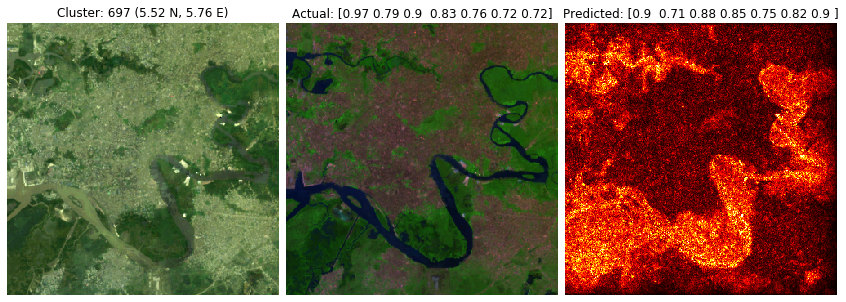
\includegraphics[width=.9\linewidth]{ig1.png} \\
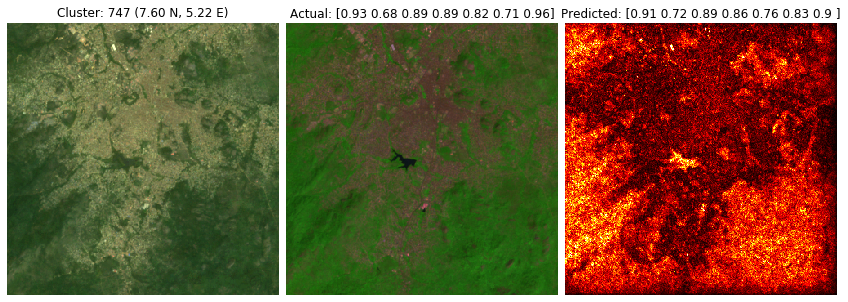
\includegraphics[width=.9\linewidth]{ig2.png} \\
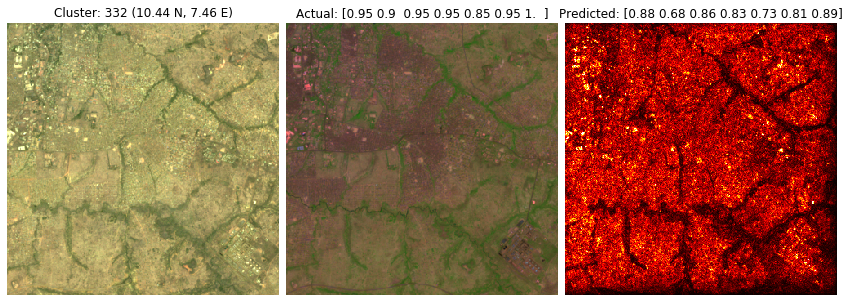
\includegraphics[width=.9\linewidth]{ig4.png} \\
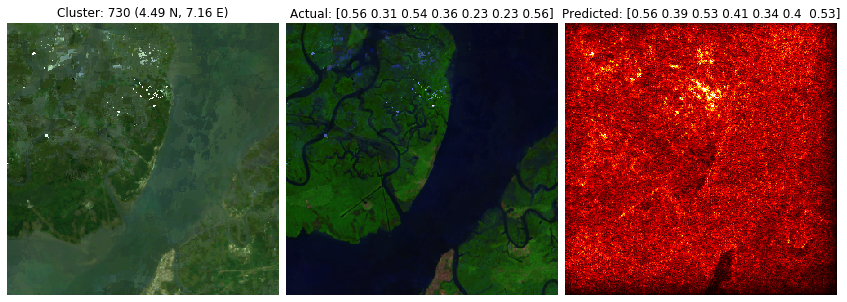
\includegraphics[width=.9\linewidth]{ig5.png} \\
\caption{The first column contains the image shown in the visible spectrum bands. The second column contains a false-color image with shortwave infrared in red (sensitive to certain types of rocks and soil), near infrared in green (sensitive to vegetation), and deep blue/violet in blue (sensitive to water). The third column shows the Integrated Gradient. Annotations above each row show cluster information, and actual/predicted vaccination rates for BCG, measles, DPT1, DPT2, DPT3, polio0, and health\_card.}
\label{fig:ig}
\end{figure}
\begin{figure}[p!]
\centering
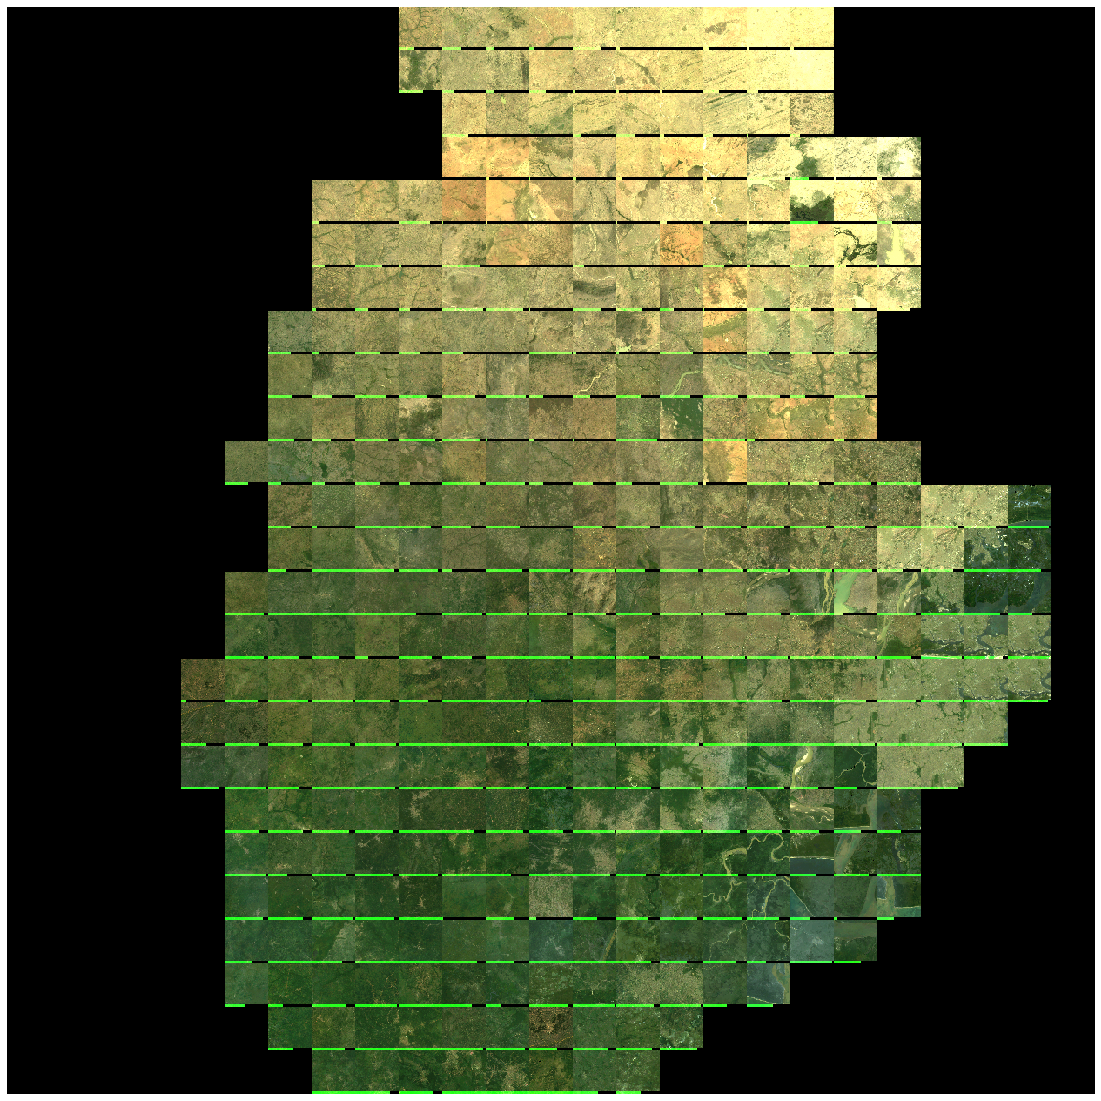
\includegraphics[width=.45\linewidth]{tsne1.png}
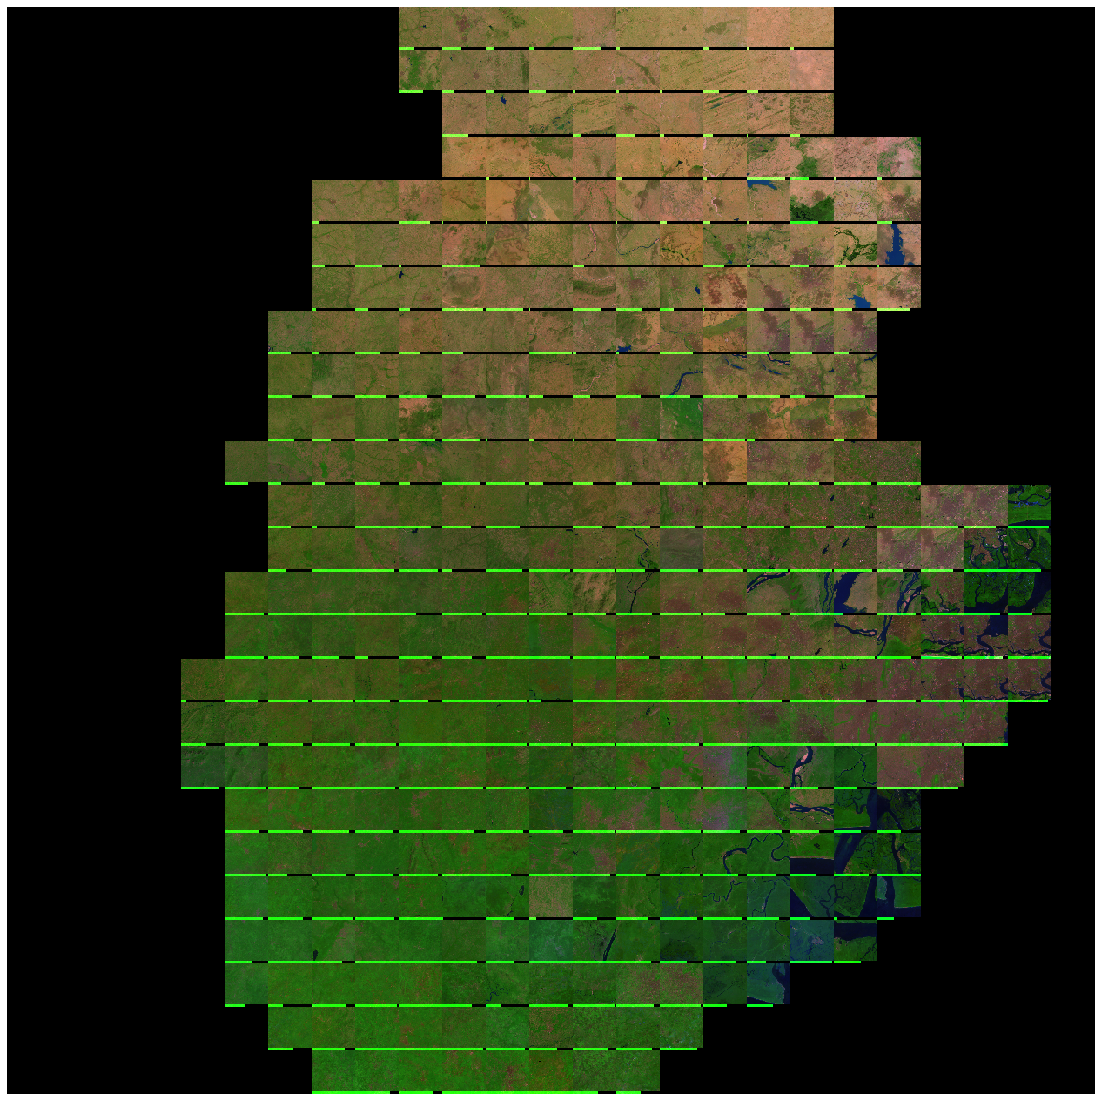
\includegraphics[width=.45\linewidth]{tsne2.png}\\
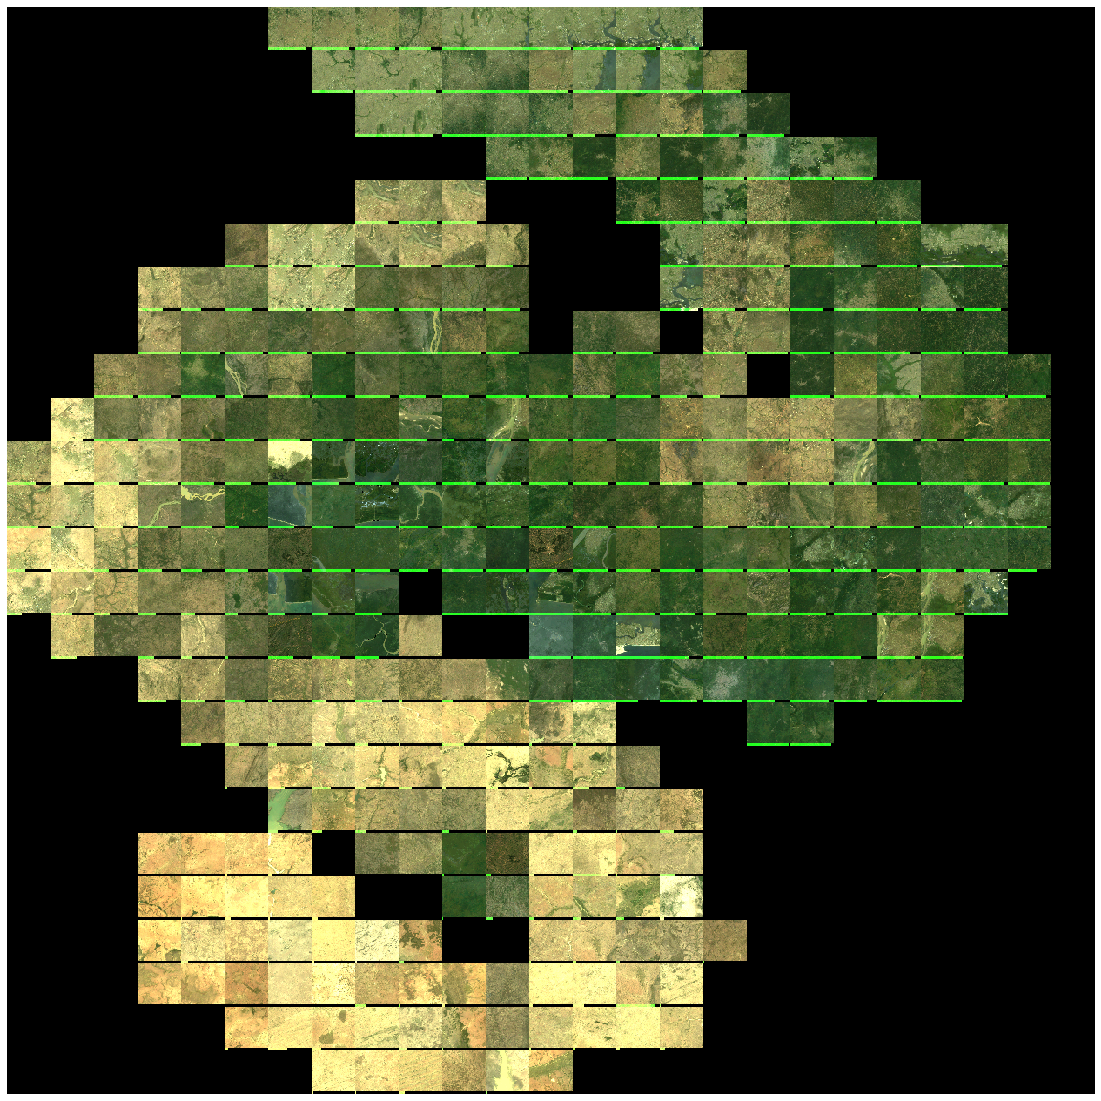
\includegraphics[width=.45\linewidth]{tsne3.png}
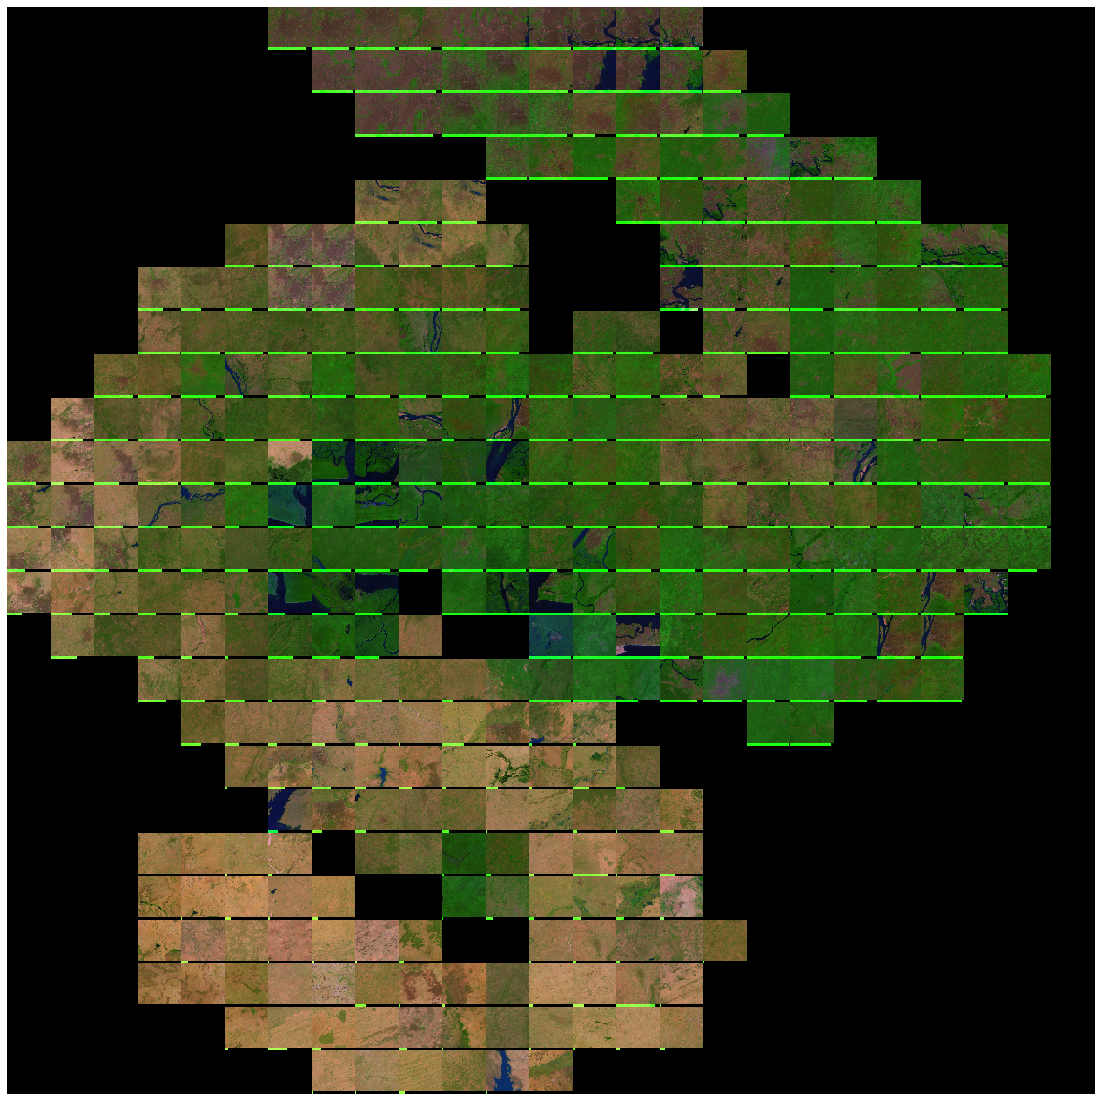
\includegraphics[width=.45\linewidth]{tsne4.png}
\caption{Image dataset visualized by embedding their extracted features using t-SNE. Green bars at the bottom of each tile show the BCG vaccination rate. The first row shows the features produced by the convolutional feature extractor, which is trained to predict nighttime light intensity. The second row shows the last hidden layer of the vaccination rate predictor. The first column shows the visible spectrum, while the second shows the false-color scheme as described in Figure \ref{fig:ig}.}
\label{fig:tsne}
\end{figure}

\subsection{Pixel Importance}
Next, we show the Integrated Gradients estimates of pixel importance in a few input images in Figure \ref{fig:ig}. These images suggest that the model is mostly picking up on visual indicators of North vs. South Nigeria.
\begin{itemize}
\item The model is sensitive to vegetation and water - both elements that are prominent in South Nigeria and not in North Nigeria. 
\item In the third row, the model appears to highlight the desertlike terrain, which again is a geographic discriminator between North and South.
\item In the fourth row, the model has a strong sensitivity to the white specks in the input, which are artifacts due to frequent cloud cover. These artifacts only appear in a region of South Nigeria which is frequently cloudy.
\end{itemize}

\subsection{Feature Embedding}
Embedding the feature vectors with t-SNE shows similar findings, which we see in Figure \ref{fig:tsne}. The feature extractor, which is trained to classify nighttime light intensity, places the most separation between the desert terrain of North Nigeria and the dense vegetation of South Nigeria. When we look at the latent features that are used to predict vaccination rates, we see a less consistent gradient of color, but it's difficult to make any conclusions beyond that.


\begin{table}[t!]
\centering
\begin{tabular}{c|cccc}
\hline
Feature \# & Lights & Lat/Lon & Built & All \\
\hline
1&45\%&56\%&32\%&74\%\\
2&47\%&53\%&36\%&73\%\\
3&48\%&43\%&42\%&69\%\\
4&45\%&49\%&38\%&70\%\\
5&44\%&61\%&31\%&76\%\\
6&47\%&53\%&36\%&74\%\\
7&48\%&51\%&40\%&74\%\\
8&45\%&54\%&32\%&71\%\\
9&47\%&50\%&38\%&72\%\\
10&47\%&45\%&40\%&69\%\\
11&43\%&53\%&34\%&72\%\\
12&45\%&52\%&35\%&71\%\\
13&42\%&55\%&30\%&71\%\\
14&46\%&53\%&36\%&73\%\\
15&45\%&57\%&33\%&74\%\\
16&51\%&50\%&42\%&75\%\\
17&45\%&42\%&38\%&66\%\\
18&45\%&60\%&32\%&77\%\\
19&48\%&59\%&34\%&78\%\\
20&48\%&54\%&38\%&75\%\\
\hline
\end{tabular}
\caption{Each feature is one of the hidden nodes in the last hidden layer of the predictor. Numbers shown are the R-squared of a linear model for each feature versus the poverty proxies listed; models are trained on the entire dataset.}
\label{table:features}
\end{table}
\subsection{Simple Predictors}
The model may be identifying signs of poverty, since impoverished areas have lower healthcare expenditure, and it has been shown that Landsat images can successfully be used to predict poverty. To test for this, we regress the latent features of our predictor against a few proxies for poverty. In addition to nighttime light intensity, we can also use latitude and longitude, as North Nigeria has higher rates of poverty than South Nigeria \cite{nigeriapoverty}; and we can use built environment from the GHSL dataset. For light intensity, we use the number of pixels classified as medium or high intensity as (two separate) features, and for GHSL, we use the number of pixels indicating built environment.

Table \ref{table:features} shows the R-squared between our latent features and the proxies for poverty. We find that a large portion of the variation in our features comes from these proxies.

We can also run this analysis on the vaccination rates directly, as shown in Table \ref{table:vaccines}. Notice that the poverty proxies have trouble predicting the same vaccines as our model. Combined with the previous analysis, this suggests that our model mostly learns the same information as the poverty proxies. However, our model generally captures more variation than the linear combination of poverty proxies.

\begin{table}[t]
\centering
\begin{tabular}{c|cccc|c}
\hline
Vaccine \# & Lights & Lat/Lon & Built & All & Our Model \\
\hline
bcg&30\%&52\%&12\%&58\%&72\%\\
measles&27\%&40\%&12\%&47\%&54\%\\
dpt1&29\%&51\%&12\%&57\%&70\%\\
dpt2&30\%&50\%&13\%&56\%&69\%\\
dpt3&30\%&46\%&13\%&53\%&64\%\\
polio0&29\%&37\%&15\%&45\%&60\%\\
polio1&15\%&24\%&7\%&27\%&17\%\\
polio2&15\%&21\%&7\%&24\%&13\%\\
polio3&5\%&5\%&3\%&8\%&0\%\\
health\_card&29\%&46\%&12\%&53\%&67\%\\
any\_vacc&12\%&22\%&7\%&24\%&13\%\\
\hline
\end{tabular}
\caption{R-squared of linear models between vaccination rates and proxies for poverty, trained on the entire dataset. The last column shows the test set R-squared of our model, for comparison.}
\label{table:vaccines}
\end{table}

\section{Conclusion and Future Work}
In this paper, we found that a CNN can be trained to predict some vaccination rates with decent accuracy. Compared to last year's Xplore project, our model has increased accuracy and lower computational costs, using Landsat 8 images instead of Google Static Maps. However, the model struggles with the same outcomes as last year - Polio1, Polio2, Polio3, and ``any vaccine''. Based on our model visualizations and regression analysis, the model seems to learn primarily economic indicators. 

\subsection{Reflection}
For this project, data collection and computational limits were the main obstacles. While Google Earth Engine greatly facilitated working with geospatial raster data, each change to the type of data needed ended up needing several hours to set up the data export task. These export tasks took about a day to run, so it was important to think ahead about what the data should look like. Then, to avoid the difficulties of using a shared computing cluster, all of the modeling was done on a local machine with limited resources; this hindered the use of deep CNN architectures. Initially, we used the MobileNet v2 architecture but were unable to get decent predictive results; switching to the less sophisticated VGG actually gave the best results. This underscored the importance of trying multiple architectures, despite differences in ImageNet accuracy. Lastly, we were able to try several ways of explaining the neural network model. For this purpose, relating the model's latent features to known variables produced the best interpretation, which is partially due to it being the simplest method.

\subsection{Future Work}
We can think of several extensions that could address some drawbacks of our analysis. 
\begin{itemize}
\item Data splitting. Some DHS clusters are very close together, so if they have similar vaccination rates, then we essentially have duplicate data in the dataset. This can create bias in our test set accuracy. It may be better to group the clusters spatially, and then separate the data at the group level.
\item Landsat images. Despite using three years of Landsat images to form our composite, we still have pixels for which there was no cloud-free image. We saw that the model is sensitive to the resulting artifacts; there may be a way to fill in these missing pixels, for example with neighboring values.
\item Choice of target for feature extractor. Since we chose to use nighttime light intensity as the classification target for training our feature extractor, it may not be a surprise that our features are highly correlated to proxies for poverty. Any sort of publicly available geospatial data could be used instead, or even a combination of outcomes trained with a combined loss.
\item Intended use of model. It is more important to accurately predict areas with low vaccination rate, so these clusters could be weighted higher during model training. We would then evaluate the model with an emphasis on these clusters.
\item Temporal map. Our initial goal was to leverage the time series of Landsat images, but we were unable to do so during the quarter. By training on multiple iterations of the DHS survey, we could produce a model which can generalize over time periods.
\end{itemize}


\bibliography{references}{}
\bibliographystyle{plain}
\end{document}
